\documentclass[10pt]{beamer}
\usepackage[utf8]{inputenc}
\usetheme{default}
\usecolortheme{dove}
\usepackage{textpos}
\usepackage{grid-system}

% \usepackage[rm]{roboto}
\usepackage[T1]{fontenc}
%\usepackage[sfdefault]{roboto}

% po4a: environment frame
% po4a: environment Row
% po4a: environment Cell

\AtBeginSection[] % Do nothing for \section*
{
	\begin{frame}<beamer>
		\frametitle{Übersicht}
		\tableofcontents[currentsection]
	\end{frame}
}

\title{\centering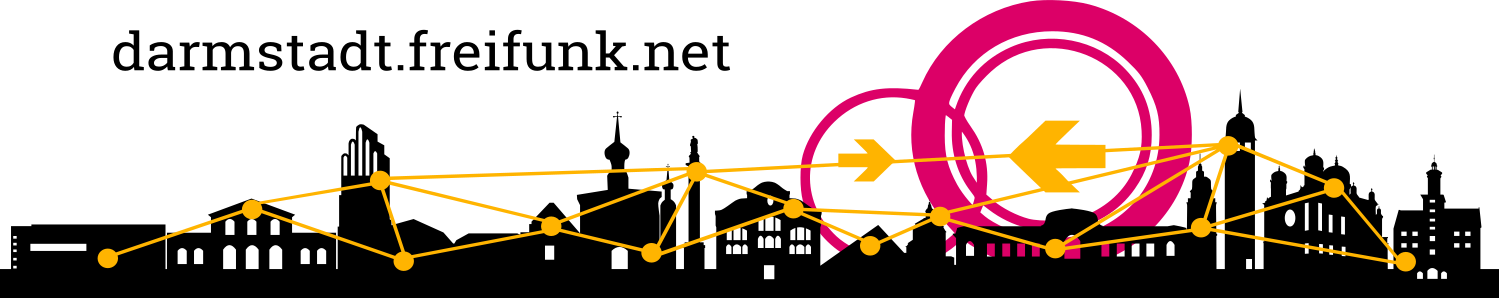
\includegraphics[width=\textwidth]{images/logo-skyline}}
\author{}
%\institute[Inst.]{Freifunk Darmstadt}
\date{\footnotesize 4. Oktober 2015}

\begin{document}


\begin{frame}
\maketitle
\end{frame}

\addtobeamertemplate{frametitle}{}{%
\begin{textblock*}{100mm}(0.92\textwidth,-0.5cm)
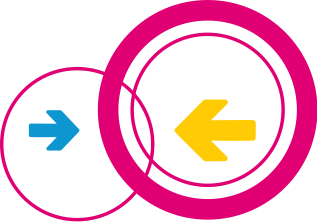
\includegraphics[height=1cm]{images/logo}
\end{textblock*}}

\begin{frame}{Übersicht}
\tableofcontents
\end{frame}

\section{Was ist Freifunk?}
\begin{frame}
	\frametitle{Was ist Freifunk?}

	Deutschlandweite Initiative für freie WLAN-Netze
	
	\pause
	\vfill
	\centering
	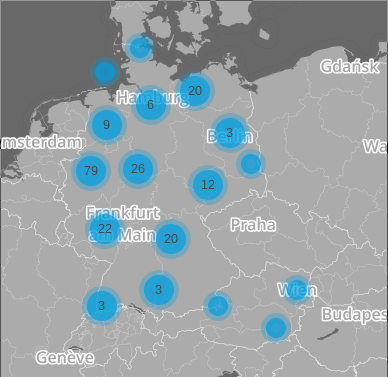
\includegraphics[scale=0.3]{images/2015-10_freifunk-map} \\
	über 200 lokale Gruppen\\bundesweit ca. 20.000 offene Zugangspunkte

	
\end{frame}

\begin{frame}
	\frametitle{Wie sieht so ein freies Netz aus?}
	\begin{center}
		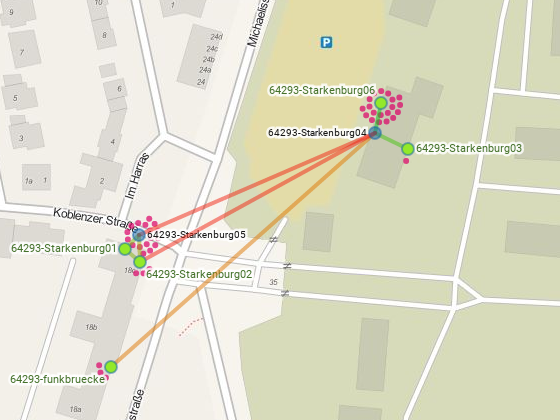
\includegraphics[height=6cm]{images/2015-08-31_starkenburg}
	\end{center}
\end{frame}

\begin{frame}
	\frametitle{Wie sieht so ein freies Netz aus?}
	\begin{center}
		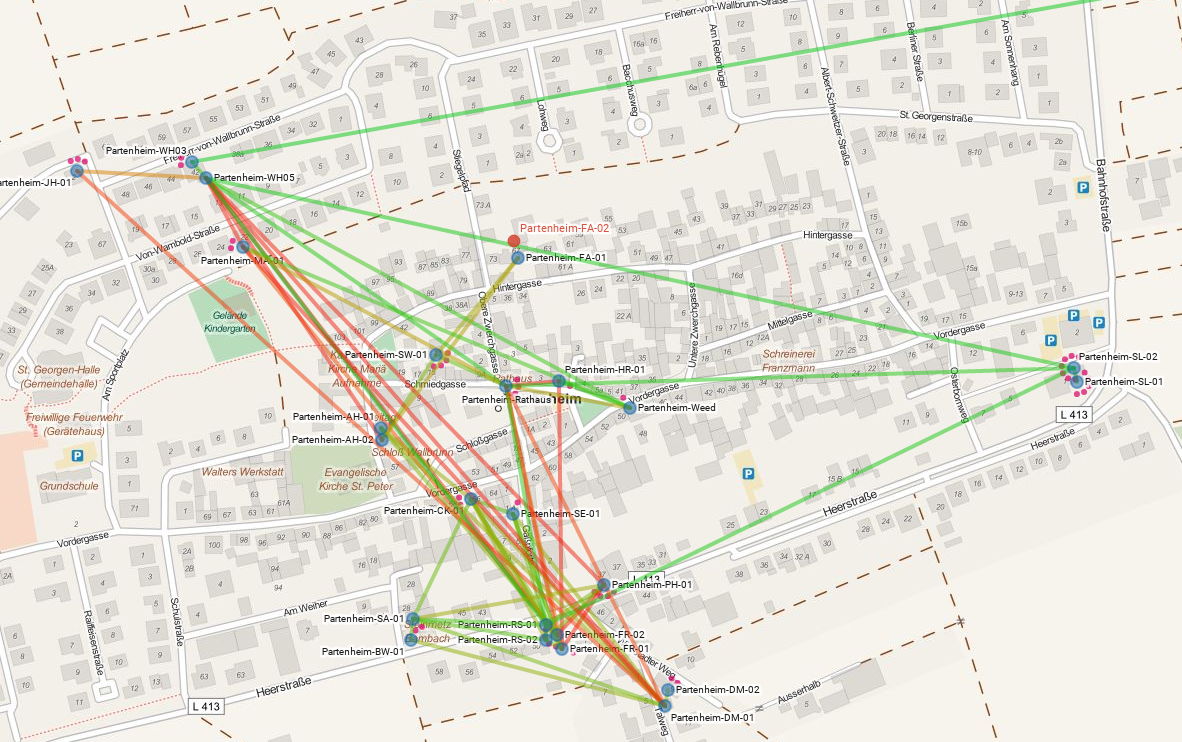
\includegraphics[height=6cm]{images/2015-10_partenheim-map}
	\end{center}
\end{frame}

\begin{frame}{Was kann man damit tun?}
	\vfill
	\begin{center}
		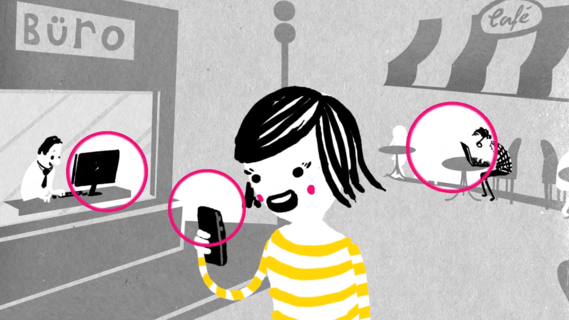
\includegraphics[width=5.5cm]{images/verbindet}
	\end{center}
	
	\begin{itemize}[<+->]
		\item jeder kann Services anbieten und nutzen
		\begin{itemize}
			\item Telefonieren und Chatten
			\item dezentrales Social-Media (z.B Diaspora, Twister)
			\item lizenzfreies Community-Radio
			\item Austausch von Dateien und Medien
			\item Blogs
			\item \ldots
		\end{itemize}
		\item gemeinsame Nutzung eines Internetanschlusses
		\item Testbed für wissenschaftliche Experimente
	\end{itemize}
	\vfill
\end{frame}

\begin{frame}
	\frametitle{Vision}
	
	Wie soll unsere Kommunikationsinfrastruktur aussehen?
	
	\begin{itemize}[<+->]
		\item offen und öffentlich
		\item anonym zugänglich
		\item nicht kommerziell
		\item dezentral organisiert
		\item unzensiert
		\item datensparsam
	\end{itemize}
\end{frame}

\begin{frame}
	\frametitle{Vision: offen und öffentlich}
	\begin{columns}[c]
		\begin{column}{5cm}
			
\includegraphics[width=\textwidth]{images/open}
		\end{column}
		\begin{column}{7cm}
			\begin{itemize}[<+->]
				\item freie, ungehinderte Teilnahme an Betrieb und Ausbau des Netzes $\Rightarrow$ Mitmachnetz
				\item Netz im (dezentralen) Besitz der Gemeinschaft
				\item freier Zugang zu Netz und Diensten
				\item keine Unterscheidung nach Ort oder Geldbeutel
			\end{itemize}
		\end{column}
	\end{columns}	
\end{frame}

\begin{frame}
	\frametitle{Vision: anonymer Zugang}
	\begin{center}
		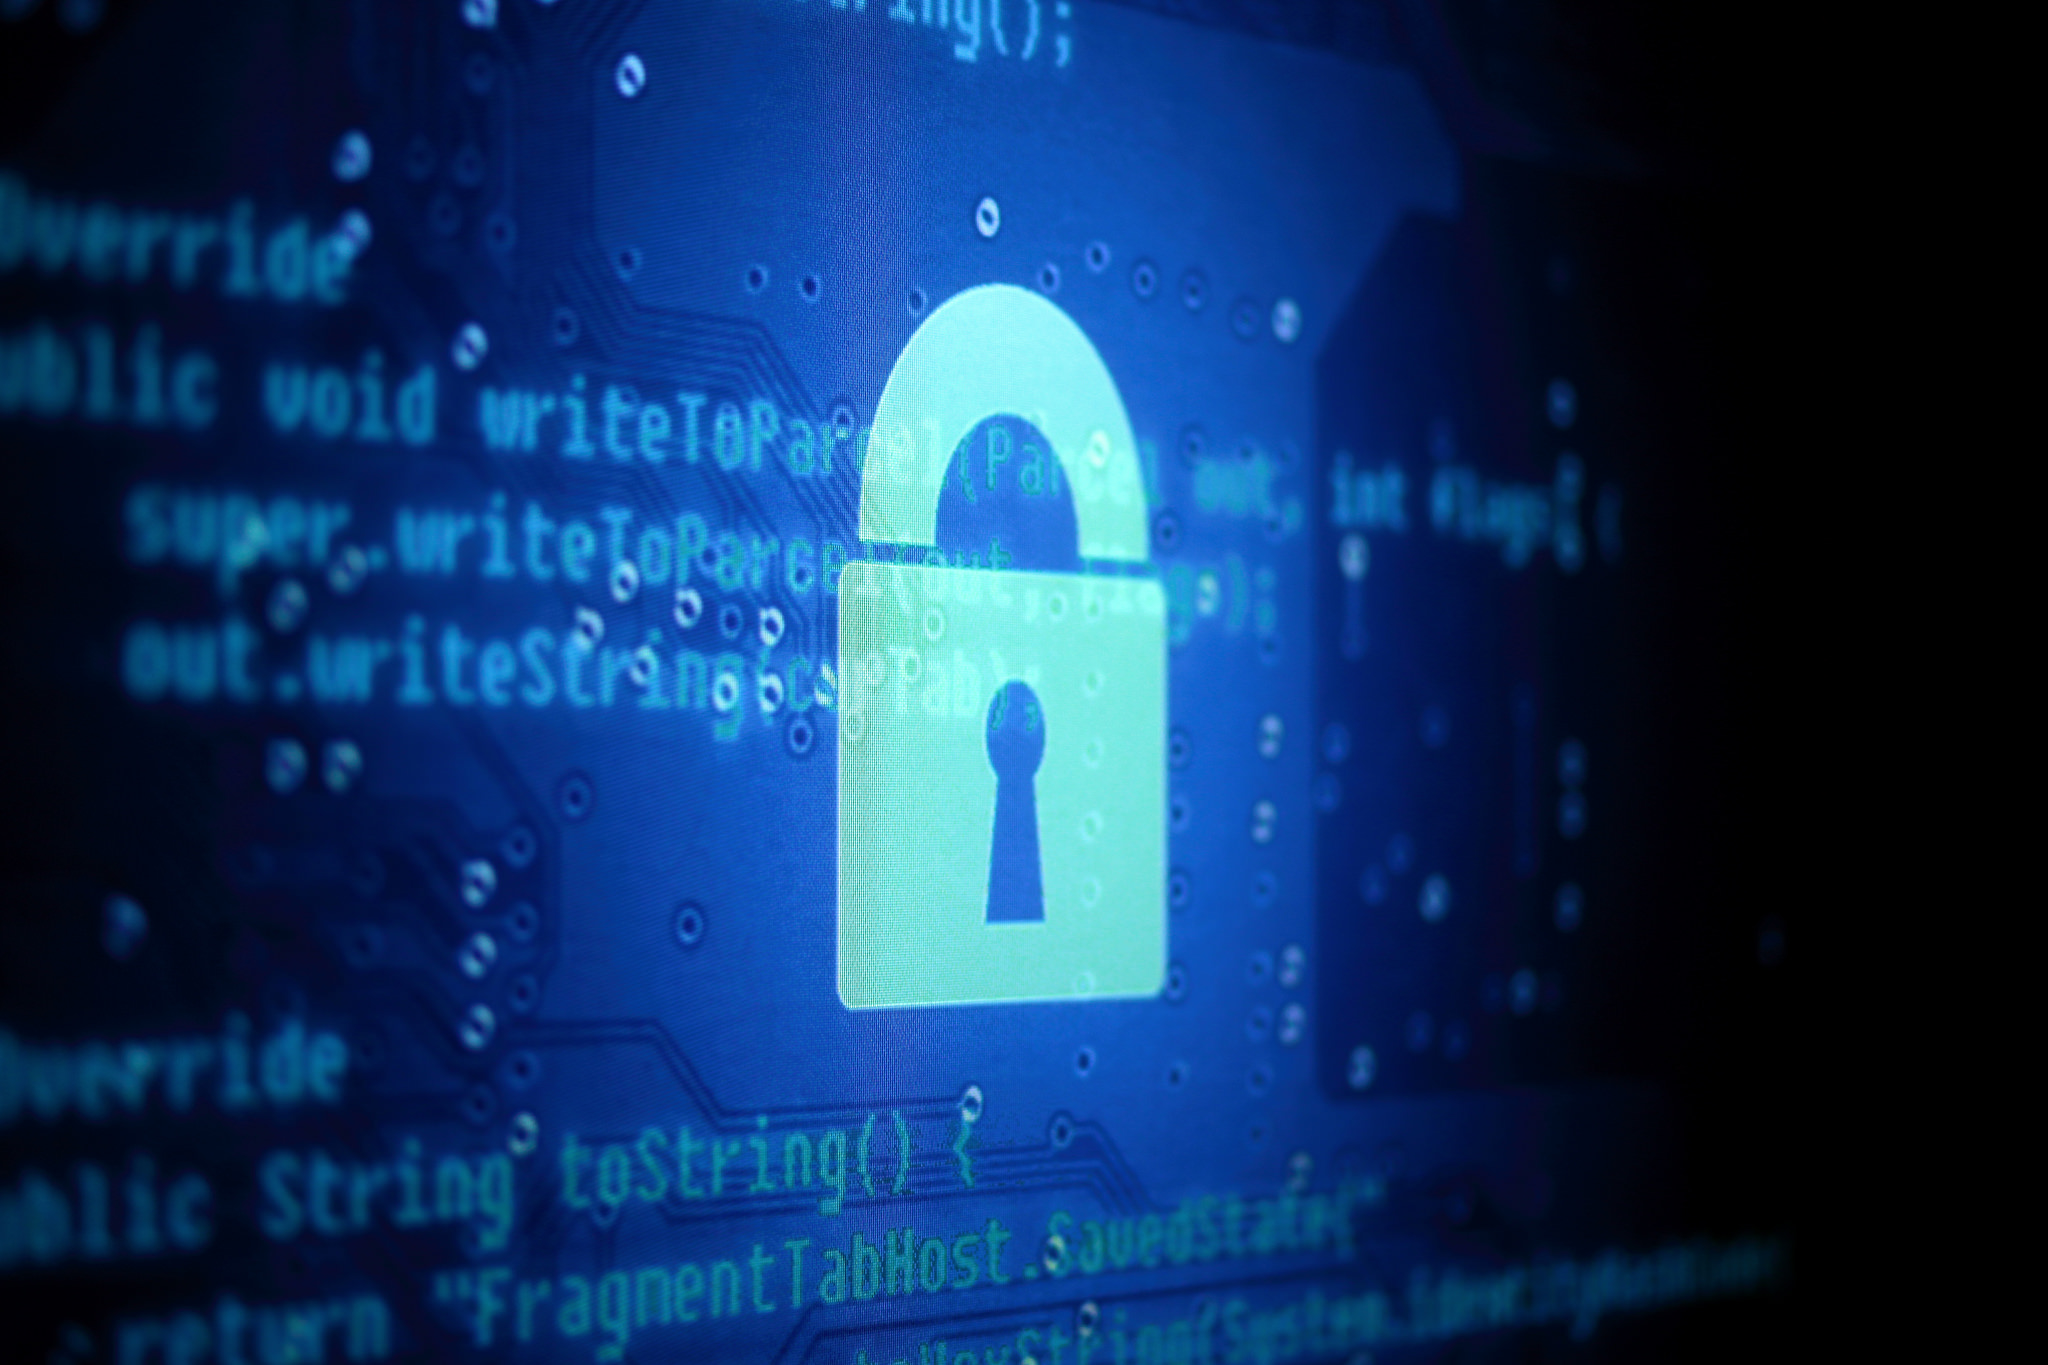
\includegraphics[width=5cm]{images/lock}
	\end{center}
	\begin{itemize}[<+->]
		\item wir verlangen keine Nutzerregistrierung
		\item Anonymer Zugang zum Netz möglich
		\item Achtung: Freifunk ist kein Anonymisierungsdienst
	\end{itemize}

\end{frame}

\begin{frame}
	\frametitle{Vision: unkommerzieller Netzbetrieb}
	\begin{columns}[c]
		\begin{column}{4cm}
			
\includegraphics[width=\textwidth]{images/non-commercial-eu}
		\end{column}
		\begin{column}{8cm}
			\begin{itemize}[<+->]
				\item kostenloser Zugang zum Freifunknetz
				\item wir verkaufen keine Benutzerdaten
				\item keine Finanzierung durch Werbung
			\end{itemize}
		\end{column}
	\end{columns}	
\end{frame}

\begin{frame}
	\frametitle{Vision: Dezentralität}
	
	\begin{itemize}[<+->]
		\item keine zentralen, für die Funktion des Netzes erforderlichen Funktionen
		\item keine Abhängigkeit von einer Gruppe von Personen
		\item Updates der Knoten durch FFDA nach Zustimmung durch die Betreiber
	\end{itemize}
	\centering
	\vfill
	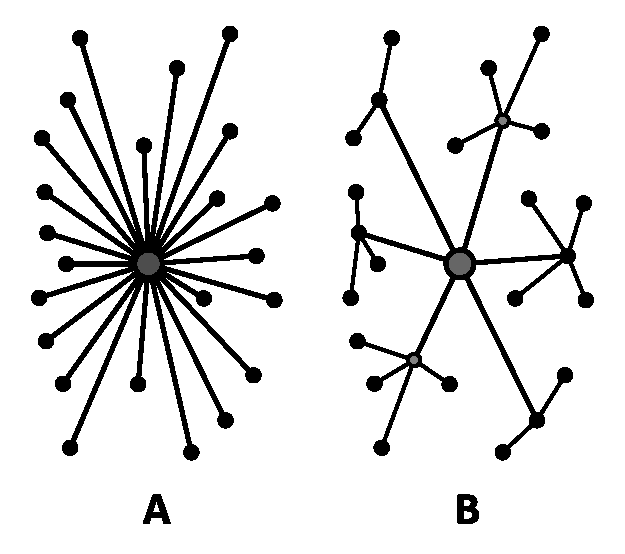
\includegraphics[width=5cm]{images/decentral}
\end{frame}

\begin{frame}
	\frametitle{Vision: Netzneutralität}
	\begin{center}
		
\includegraphics[width=0.7\textwidth]{images/netneutrality}
	\end{center}
	Alle Daten werden gleichberechtigt übertragen:
	\begin{itemize}[<+->]
		\item keine Filterung der Inhalte
		\item keine Zensur
		\item keine Priorisierung
	\end{itemize}

	% Bilder dezentrales mesh, zustimmung
\end{frame}

\begin{frame}
	\frametitle{Vision: Datensparsamkeit}
		\begin{columns}[c]
			\begin{column}{5cm}
				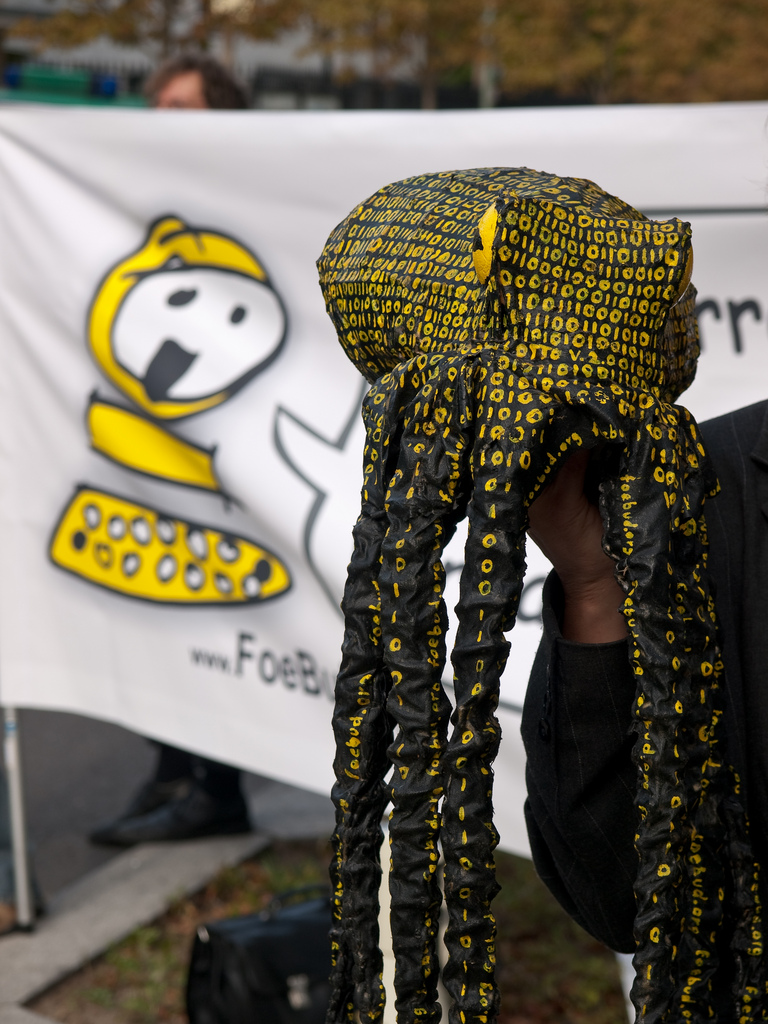
\includegraphics[width=\textwidth]{images/krake}
			\end{column}
			\begin{column}{7cm}
				\begin{itemize}[<+->]
					\item keine Sammlung von Verbindungs- oder Verkehrsdaten
					\item keine persönlichen Stammdaten
					\item freiwillige Angabe von Kontaktdaten und Ort eines Knoten
				\end{itemize}
			\end{column}
		\end{columns}
\end{frame}

\begin{frame}
	\frametitle{Ziele von Freifunk}
	\begin{itemize}[<+->]
		\item Verständnis von Datennetzen sowie deren Auswirkungen auf die Gesellschaft fördern
		\item Teilnahme der Bevölkerung an Forschung und Aufbau dezentraler Netze
		\item unser Wissen und Software öffentlich zugänglich machen
		\item Beteiligung an politischen Prozessen, um die rechtlichen Voraussetzungen für freie Netze zu schaffen
	\end{itemize}
\end{frame}

\section{Wie funktioniert Freifunk?}

\begin{frame}{Ohne Freifunk}
	\begin{center}
		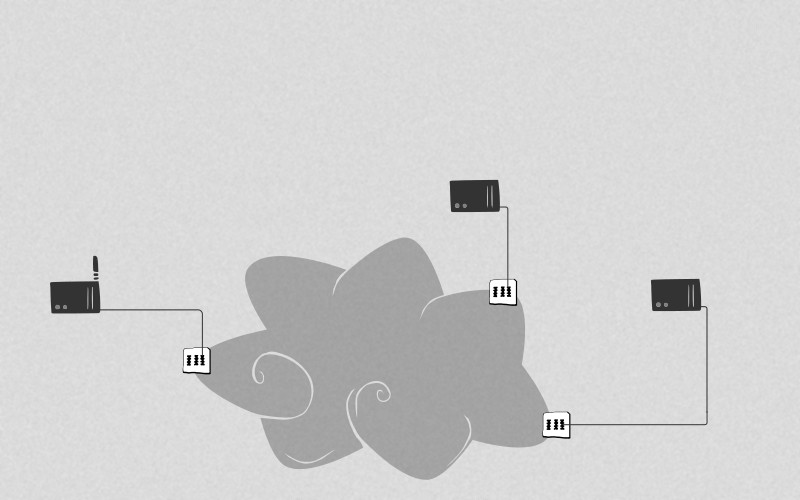
\includegraphics[height=6cm]{images/network_1} \\
		\vfill
		Viele geschlossene (WLAN-)Netze, die nicht miteinander kommunizieren
	\end{center}
\end{frame}

\begin{frame}{Mit Freifunk}
	\begin{center}
		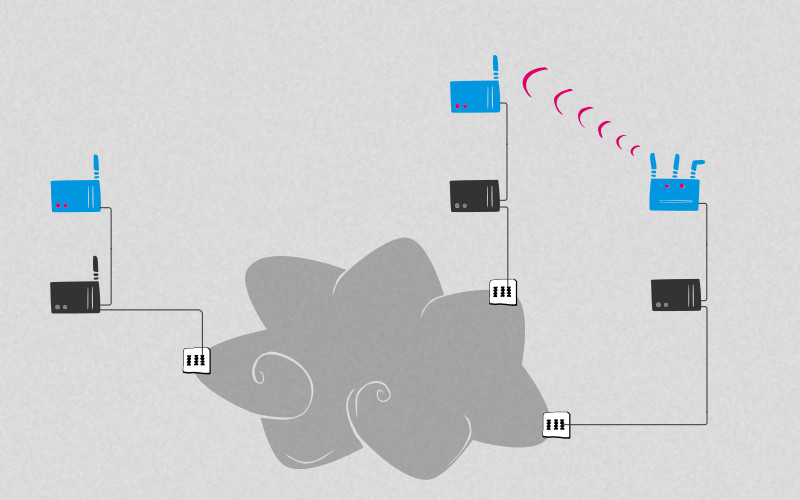
\includegraphics[height=6cm]{images/network_2} \\
		\vfill
		Freifunkknoten bauen ein lokales Netz auf
	\end{center}
\end{frame}

\begin{frame}{Verminderung der digitalen Kluft}
	\begin{center}
		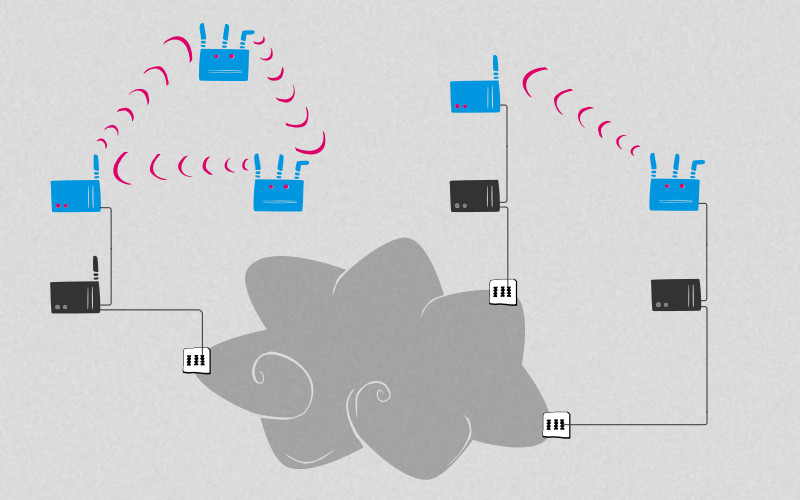
\includegraphics[height=6cm]{images/network_3} \\
		\vfill
		Das Freifunknetz kann mit neuen Knoten erweitert werden,\\ auch dort, wo es keine Internetzugänge gibt
	\end{center}
\end{frame}

\begin{frame}{Das Heimnetz bleibt privat}
	\begin{center}
		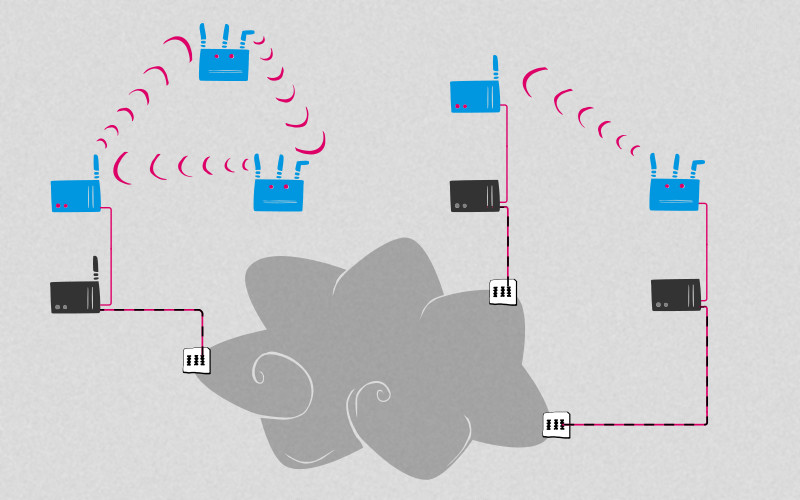
\includegraphics[height=6cm]{images/network_4} \\
		\vfill
		Eigenes Heimnetz und Freifunk-Netz sind getrennt
	\end{center}
	
\end{frame}


\begin{frame}{Zugang zum Internet}
	\begin{center}
		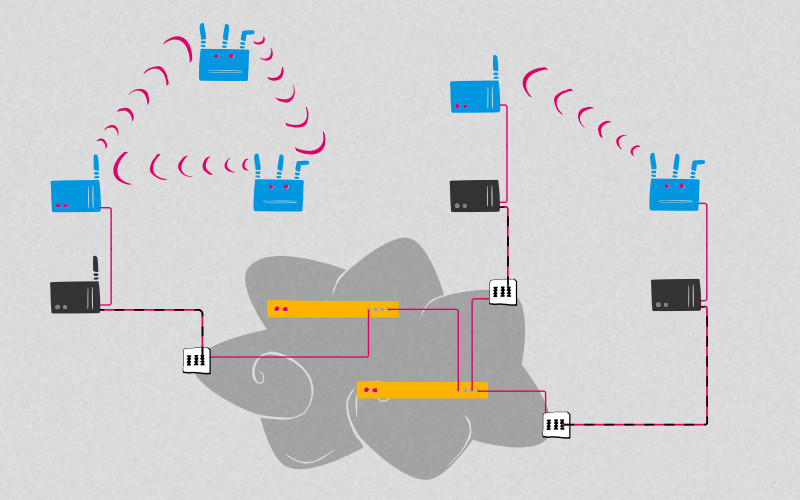
\includegraphics[height=6cm]{images/network_5} \\
		\vfill
		Daten aus dem Freifunknetz werden erst durch unsere Gateways\\ ins Internet weitergeleitet
	\end{center}
\end{frame}

\section{Rechtliche Aspekte und Risiken}

\begin{frame}{Internet teilen vs. Störerhaftung}
	
	\begin{columns}[c]
		\begin{column}{4cm}
			
\includegraphics[width=\textwidth]{images/recht}
		\end{column}
		\begin{column}{8cm}
	\begin{itemize}
		\item Teilen des eigenen Internetanschlusses ist in Deutschland legal
		\pause\item \textbf{aber:} Mithaftung für illegale Aktivitäten, wenn Täter nicht zu ermitteln ist
		\pause\item Abmahnkosten sind zu tragen
	\end{itemize}
	
	\bigskip
	\pause
	
	Unsere Lösungen:
	\begin{itemize}
		\item VPN in Länder ohne Störerhaftung
		\item selbst Internetanbieter werden
	\end{itemize}
		\end{column}
	\end{columns}
	
	\vfill
	\centering
	\pause \textbf{Fazit:}\\Störerhaftung existiert noch, wir machen es aber sehr schwer,\\den eigentlichen Anschlussinhaber zu finden.

\end{frame}

\begin{frame}{Sicherheit im Freifunk-Netz}
	\begin{itemize}[<+->]
		\item Freifunk als freies Netz bietet keinen Schutz
		\item WLAN ist nicht verschlüsselt, vertrauliche Daten nur mit Ende-zu-Ende-Verschlüsselung (z.B. https) übertragen
		\vfill
		\item Daten im Freifunk-Netz: Gesamter Verkehr schwer zu überwachen
		\pause\item Daten ins Internet: Betreiber der Gateways können überwachen
		\vfill
	\end{itemize}
	\centering
	\textbf{Fazit:}\\Zentrale Überwachung und Zensur deutlich schwieriger als im Internet, \\
	Benutzer sind selbst verantwortlich für Schutz und Verschlüsselung.
\end{frame}

\section{Freifunk in Darmstadt}

\begin{frame}{Freifunk Darmstadt (FFDA)}
	\begin{columns}[c]
		\begin{column}{4cm}
			
\includegraphics[width=\textwidth]{images/cda}
		\end{column}
		\begin{column}{8cm}
			\begin{itemize}
				\item Projekt des Chaos Darmstadt e.V., Erfa-Kreis des CCC
				\item 13. Februar 2014: erstes FFDA-Treffen
			\end{itemize}
		\end{column}
	\end{columns}
\end{frame}
\begin{frame}{1.x Jahre FFDA-Netz}
	\vfill
	\begin{itemize}[<+->]
		\item 26. Juni 2014: erster Knoten geht online
		\item vor einem Jahr: ca. 30 Knoten
		\item heute: 280 Knoten, davon ca. 215 online
	\end{itemize}
	\pause
	\begin{center}
		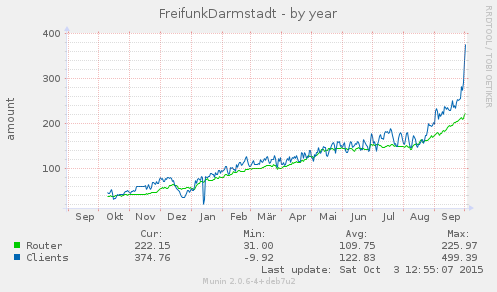
\includegraphics[width=0.8\textwidth]{images/ffda-Okt14-15}
	\end{center}
\end{frame}

\begin{frame}{Stand Oktober 2015}
	\begin{center}
		\vfill
		ca. 220 Knoten, über 400 Clients
		\begin{center}
			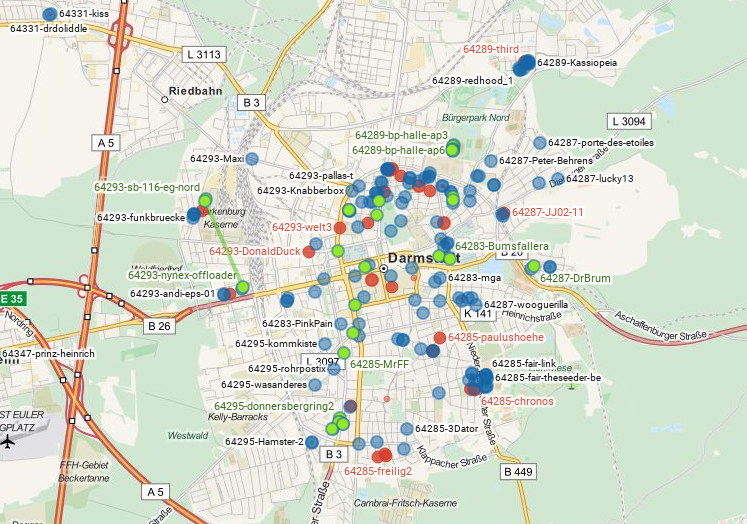
\includegraphics[width=0.7\textwidth]{images/2015-10-03_darmstadt-map}
		\end{center}
		
		\vfill
		\url{https://map.darmstadt.freifunk.net}
		
		\tiny oder \url{https://map.ffda} im Freifunk-Netz
	\end{center}	
\end{frame}

\begin{frame}{Aktuelle Aufgaben}
	\begin{center}
		\large Flüchtlingsheime mit Internet versorgen \\
		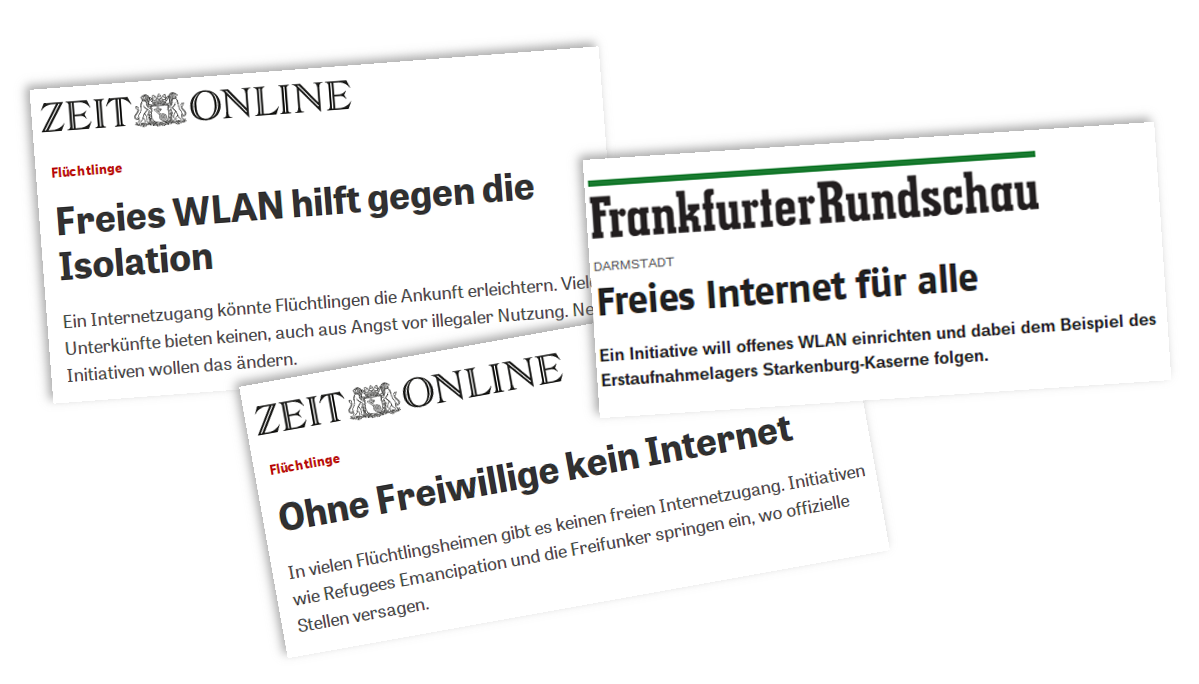
\includegraphics[width=0.7\textwidth]{images/2015-10_presse-fluechtlinge}
	\end{center}
	\begin{itemize}[<+->]
		\item in Darmstadt: Starkenburg Kaserne, Donnersbergring, Sporthalle am Nordbad
		\item auch in Eberstadt, Biebesheim, Stockstadt am Rhein
		\item hoffentlich bald: Seeheim-Jugenheim, Wixhausen, Mühltal
	\end{itemize}	
\end{frame}	

\begin{frame}{Aktuelle Aufgaben}
	\begin{center}
		\large Öffentlichkeitsarbeit
		\vfill
	\end{center}
	\begin{itemize}[<+->]
		\item Kontakt mit:
		\begin{itemize}[<+->]
			\item der Stadt Darmstadt und anderen Städten im Landkreis
			\item politischen Parteien
			\item Presse
			\item Bewohner
			\item NGOs, Vereine, Schulen, \ldots
			\item Cafés, Hotels, Geschäfte, \ldots
		\end{itemize}
		\vfill
		\item Vorträge und Workshops organisieren
		\vfill
		\item Sponsoren finden für Technik und öffentliche APs
	\end{itemize}
\end{frame}

\begin{frame}{Aktuelle Aufgaben}
	\begin{center}
		\large Netzwerkwartung
		\vfill
	\end{center}
	\begin{columns}[T]
		\begin{column}{5cm}
			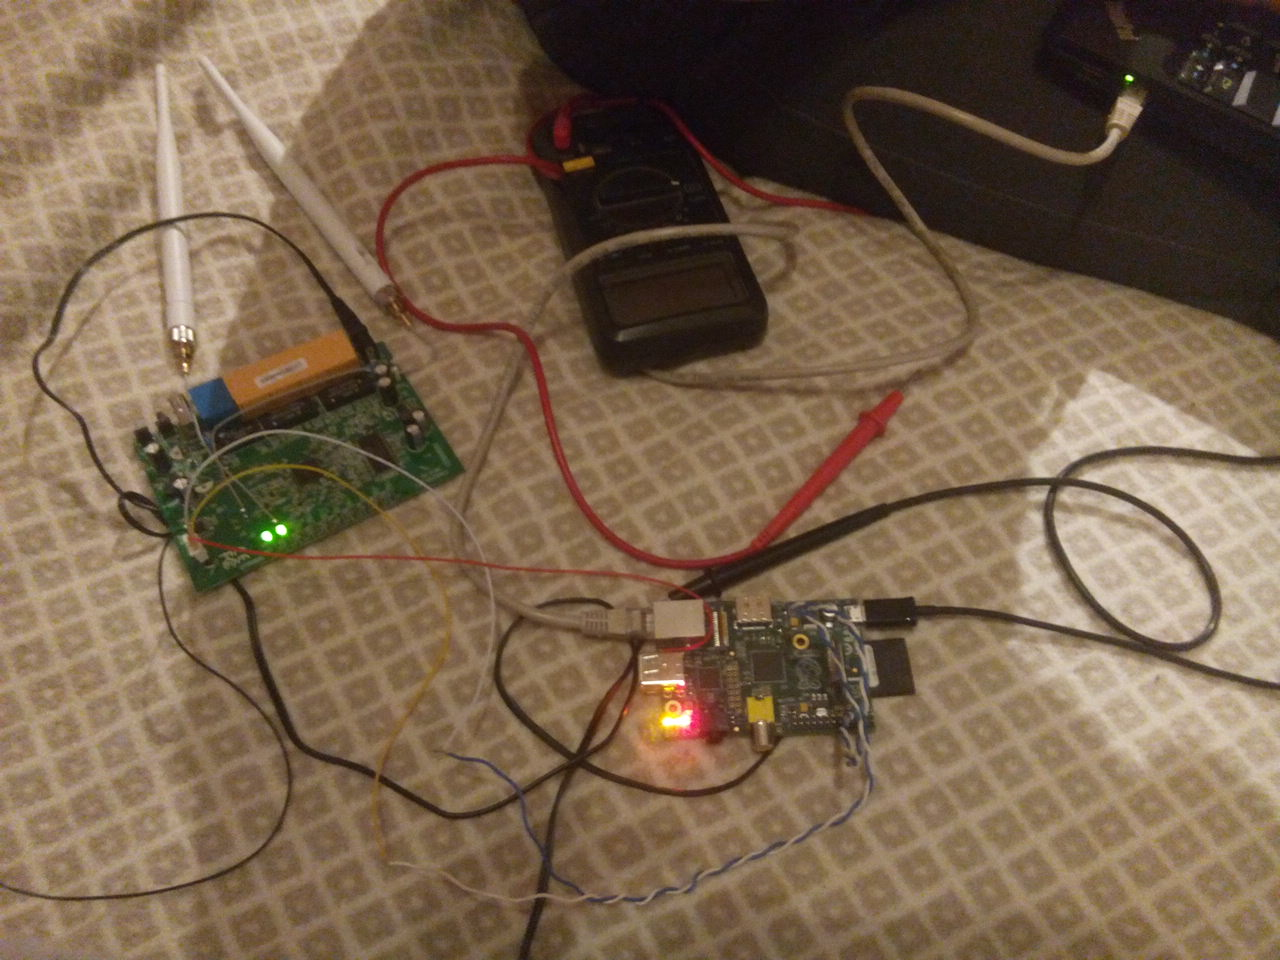
\includegraphics[width=\textwidth]{images/disassemble}
		\end{column}
		\begin{column}{7cm}
			\begin{itemize}[<+->]
				\item neue Firmware für Knoten
				\item Analyse des Netzwerkstatus und Reaktion bei Problemen
				\item Betrieb der Gateways ins Internet
				\item Verbindung zu anderen Communities
				\item Experimente mit unterschiedlichen Protokollen, Software und Hardware
			\end{itemize}
		\end{column}
	\end{columns}
\end{frame}

\begin{frame}{Wir freuen uns auf Freiwillige}
	\begin{itemize}
		\item ca. 7 Menschen im Kernteam
		\item viel Arbeit seit Unterbringung der Flüchtlinge
		\vfill
		\item wir Treffen uns jeden Montag um 19 Uhr
		\item außerdem online im IRC (\#ffda @ hackint.org)
		\item andere Kontaktmöglichkeiten auf unserer Webseite
	\end{itemize}
\end{frame}

\begin{frame}{Q~\&~A}
\vfill
\centering
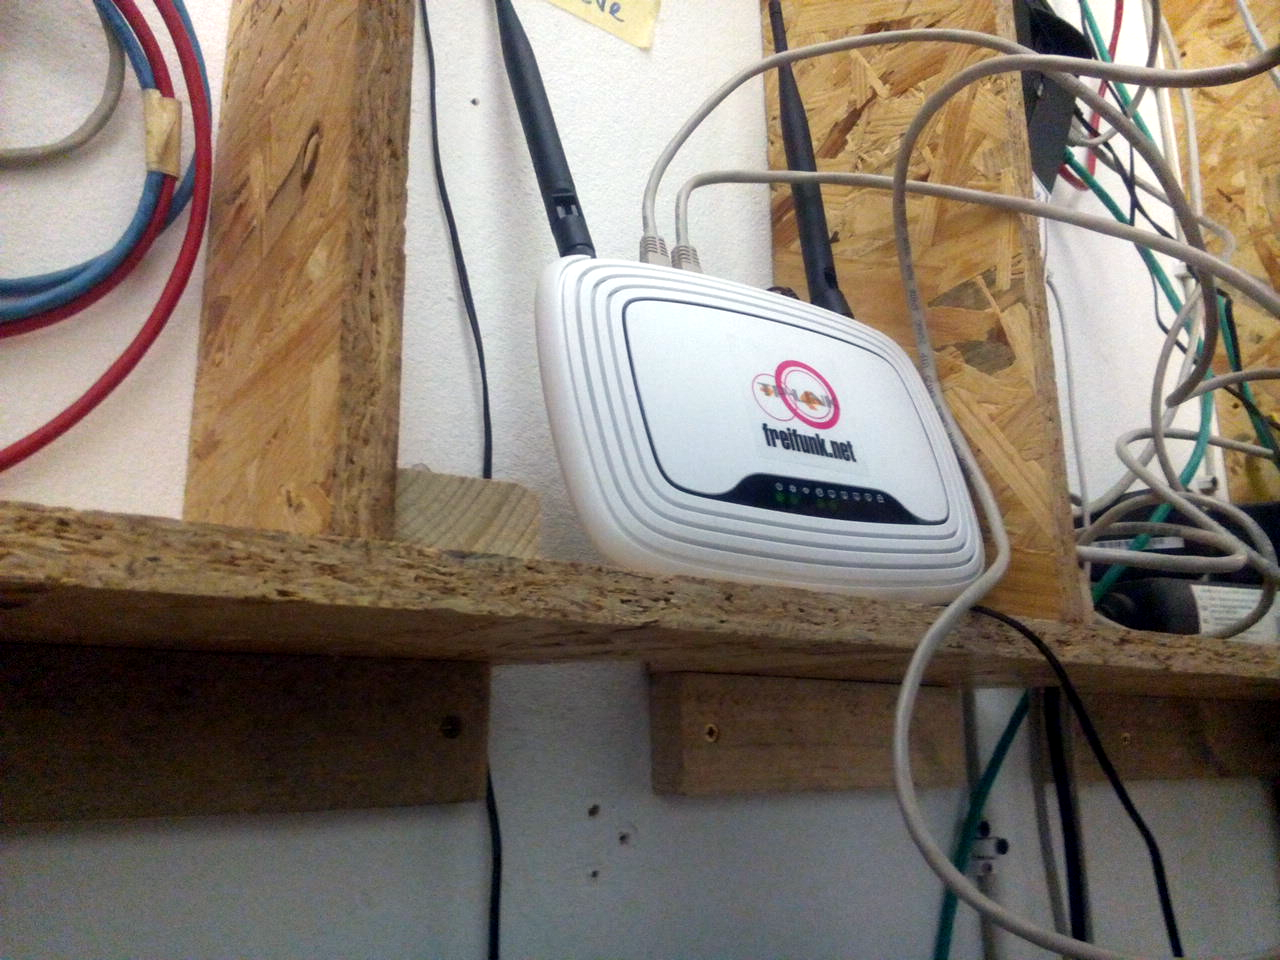
\includegraphics[width=0.7\textwidth]{images/irl_router}
\vfill
\end{frame}

\begin{frame}{Quellen}
\url{https://www.flickr.com/photos/29355306@N06/15613972489/}\\
\url{https://www.flickr.com/photos/yusamoilov/13334048894}\\
\url{https://www.flickr.com/photos/dbaron/2771996590/}
\end{frame}


\end{document}
